\documentclass{exam}
\usepackage[utf8]{inputenc}
\usepackage{color}
\usepackage{amsmath}
\usepackage[english]{babel}
\usepackage{comment}
\usepackage{graphicx}
\usepackage{caption}
\usepackage{subcaption}
\usepackage[siunitx]{circuitikz}
\newcommand{\splitcell}[2][c]{%
  \begin{tabular}[c]{@{}c@{}}\strut#2\strut\end{tabular}%
}
\usepackage{natbib}
\usepackage{listings}
\usepackage{xparse}
\usepackage{hyperref}
\usepackage{float}
\usepackage{tcolorbox}

\NewDocumentCommand{\codeword}{v}{%
\texttt{\textcolor{blue}{#1}}%
}
\usepackage{pgfplots}
\pgfplotsset{compat = newest}
\usepackage{chngcntr}
\counterwithin{table}{section}
\counterwithin{figure}{section}

\usepackage{listings}
\usepackage{xcolor}

\definecolor{codegreen}{rgb}{0,0.6,0}
\definecolor{codegray}{rgb}{0.5,0.5,0.5}
\definecolor{codepurple}{rgb}{0.58,0,0.82}
\definecolor{backcolour}{rgb}{0.95,0.95,0.92}

\lstdefinestyle{mystyle}{
    backgroundcolor=\color{backcolour},   
    commentstyle=\color{codegreen},
    keywordstyle=\color{magenta},
    numberstyle=\tiny\color{codegray},
    stringstyle=\color{codepurple},
    basicstyle=\ttfamily\footnotesize,
    breakatwhitespace=false,         
    breaklines=true,                 
    captionpos=b,                    
    keepspaces=true,                 
    numbers=left,                    
    numbersep=5pt,                  
    showspaces=false,                
    showstringspaces=false,
    showtabs=false,                  
    tabsize=2
}

\lstset{style=mystyle}

\begin{document}

\newcommand{\Exjobbsnummer}[1]{
	\begin{tikzpicture}[overlay, remember picture]
		\path (current page.north east) ++(-1,-1) node[below left] {{\small #1}};
	\end{tikzpicture}
}

\newcommand{\Examensjobbspoang}[1]{
	\begin{tikzpicture}[overlay, remember picture]
		\path (current page.north east) ++(-1,-1.5) node[below left] {{\normalsize \scshape Examensarbete #1 HP}};
	\end{tikzpicture}
}

\newcommand{\datum}[1]{
	\begin{tikzpicture}[overlay, remember picture]
		\path (current page.north east) ++(-1,-2.0) node[below left] {{\normalsize #1}};
	\end{tikzpicture}}

\newcommand{\storlitentitel}[2]{
\center
\rule[0.2cm]{13cm}{0.1cm}
{ \huge \bfseries #1}\\[0.4cm] % Title of your document
{\Large \slshape #2}\\[0.4cm]
\rule[0.2cm]{13cm}{0.1cm}\\[3cm]

}

\newcommand{\Namn}[2]{
	\begin{minipage}{0.5\textwidth}
		\normalsize
		\centering
		#1 \textsc{#2}\\
	\end{minipage}\\
}

\newcommand{\LoggaSwe}{
	\textsc{\Huge Internet Performance \\[0.3cm] and Troubleshooting Lab}\\[0.7cm]
	
\includegraphics[scale=.06]{polito_logo_2021_blu.jpg}\\[1.5cm]
}

\newcommand{\LoggaEng}{
	\textsc{\Huge Uppsala University}\\[0.7cm]
	\includegraphics[scale=.1]{Uppsala_University_seal_svg.png}\\[0.5cm]
}

% -----------------------------------------------
%           HÄR BÖRJAR TITELSIDAN
%------------------------------------------------
\begin{titlepage}

	\center

	%-------------------------------------------------
	%	INFORMATION ATT FYLLA I
	%-------------------------------------------------
	\Exjobbsnummer{Academic Year 2023/2024}
	%\datum{2021/2022}

	\LoggaSwe
	% \LoggaEng - Byt till engelska

	\storlitentitel{\\Report II}{Analysis of Chargen}

	\Large Group 3\\
	\Namn{Brendon Mendicino}{(s317639)}
	\Namn{Alessandro Ciullo}{(s310023)}
	\Namn{Davide Colaiacomo}{(s313372)}

	\vfill

\end{titlepage}
\pagebreak

\section{Network Configuration}

The network configuration used during the experiments is the following:
\begin{figure}[H]
    \centering
    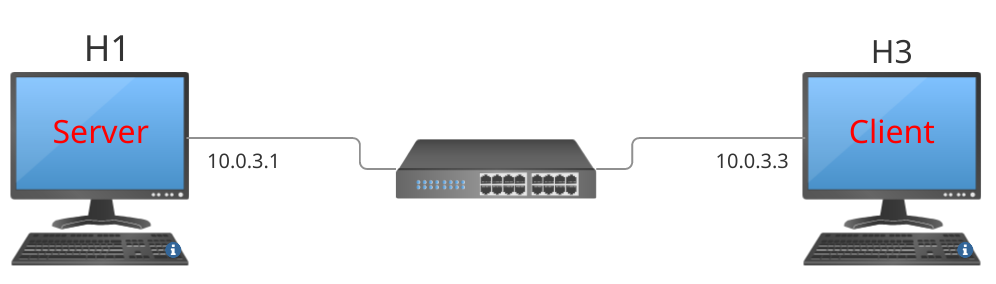
\includegraphics[width=0.75\linewidth]{network-topology.png}
    \caption{Enter Caption}
    \label{fig:enter-label}
\end{figure}
\begin{table}[h!]
  \begin{center}
    \begin{tabular}{|l|l|l|}
      \hline
      \textbf{Host name} & \textbf{IP address} & Role \\
      \hline
      H1 & 10.0.3.1/25 & Server \\
      \hline
      H3 & 10.0.3.3/25  & Client \\
      \hline
    \end{tabular}
  \end{center}
  \caption{Net hosts}\label{tab:net-hosts}
\end{table}

\section{Chargen experiment: A Macroscopic view}
\subsection{How chargen works}
Chargen is a character generator protocol standardized by RFC 864. The popular pattern works by sending lines composed of 72 characters taken from a sliding window over a circular buffer of 95 printable characters and terminated with \verb|\r\n| for a total of 74 bytes per line. 

\subsection{The experiment steps}
The following experiment aims to analyze how the fields of the \textbf{TCP} header change over time during a connection between a \verb|Chargen server| and a \verb|client|.

The first experiment was performed by executing a series of actions on the client-side, each separated by a 5 seconds delay, in the following order:
\begin{enumerate}
    \item create a connection to the Chargen server, using the \verb|Telnet| protocol.
    \item try to decrease the size of the terminal window.
    \item try to increase the size of the terminal window.
    \item press the key combination \verb|^C| on the client terminal.
    \item press the key combination \verb|^]| on the client to access the \verb|Telnet| console.
    \item press the \verb|Enter| key on the client to resume the connection.
    \item press the key combination \verb|^]| on the client.
    \item close the connection through the command \verb|telnet> quit|.
\end{enumerate}
As it noticeable in Figure~\ref{fig:ack}, the first 10 seconds (step 2 and 3) do not show any noticeable change in the slope of the graph; this means that resizing the window is not enough to cause a slowdown of the throughput as we expected and, actually, we'll find out a completely different result in the corresponding microscopic view of the experience.

When the client presses \verb|^C|, Telnet will send some bytes to the server, which will represent the command ASCII notation of \verb|^C +\r\n| (5 bytes corresponding to the only grow in the client sequence number), on top of that telnet will stop printing characters on screen, this will cause (probably) telnet to dump the bytes got from the socket instantly, thus causing the TCP buffer to get emptied faster that what the server is able to send to the client. For this reason we can see that the angle of the curve in the interval $[10s, 15s]$ is much greater than before, this means that the data being sent by the server to the client is much greater than before. This is further confirmed by the \textbf{Throughput Graph} shown in Wireshark Figure~\ref{fig:throughput} which reaches $0.8Gb/s$.
After this phase we press the  \verb|^]| combination and pass to the telnet terminal: this gradually interrupts the communication and will mark the beginning of a waiting procedure that we addressed as the \textbf{Keep-Alive} phase and analyzed it later in the report. Than we resumed the communication by pressing \verb|Enter| and observed the same behavior of the \verb|^C| phase till we returned in the telnet terminal mode and by writing \verb|quit| we closed the connection. 


From analysing the Figure~\ref{fig:win} it's also noticeable that the server segment size is always changing, in the first 10 seconds this is explained by the fact that the server reaches the full size of the Client window, which implies that the segment will be truncated earlier than the MSS. This is fluctuation in the segment size is also present in the \verb|^C| phase where the client receiving window is never saturated; the reason behind this is in the implementation of Chargen: the application makes use of the \verb|PUSH| flag to delimit and push sets of completed lines. During the first part of the experiment in fact the sum of data from a push to the next one was always a multiple of 74 (justifying the truncation) but later even if this synchrony for what we thinks are implementation reasons this behavior continue.


One last thing to be noted is that, when the connection is closed at the end of the experiment (step 8), the Chargen server sends a \textbf{FIN/ACK} fragment to request the termination of the connection, then immediately sends a \textbf{RST/ACK} fragment without actually waiting for any acknowledgement for the former, leading to a connection shutdown without further availability from the server to receive any client's packets related to the current connection.

\section{Chargen experiment: A Microscopic view}
\subsection{The handshake phase}
As the connection between the Chargen server and the client relies on TCP, it is appropriate to dive deeper into the establishment of the connection between them. Taking for granted that the following packets all carry a 14 bytes \verb|Ethernet header|, a 20 bytes \verb|IP header| and a 20 bytes \verb|TCP header| plus the \verb|TCP options|, figure \ref{fig:wireshark-three-way_handshake} shows, as expected according to the \verb|three-way handshake| procedure, that:
\begin{enumerate}
    \item the client starts sending a 74 bytes \textbf{SYN} fragment to the Chargen server.
    \item the Chargen server answers back to the client with a 74 bytes \textbf{SYN/ACK} fragment.
    \item the client finally answers back to the Chargen server with a 66 bytes \textbf{ACK} fragment.
\end{enumerate}
\begin{figure}[H]
    \centering
    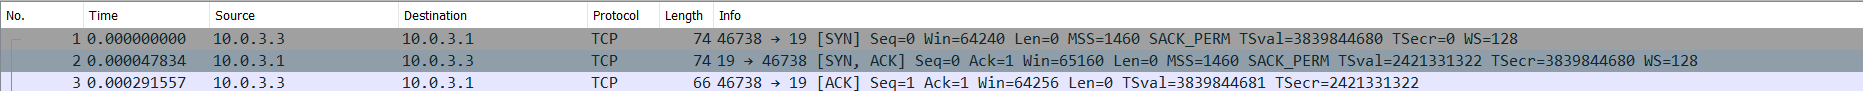
\includegraphics[width=0.90\textwidth]{three_way_handshake.png}
    \caption{Wireshark - Three-way Handshake}
    \label{fig:wireshark-three-way_handshake}
\end{figure}

\subsubsection{SYN fragment (client $\rightarrow$ server)}
Figure \ref{fig:syn_fragment} shows that the \verb|source port| is a random one picked above the well-known ports (0-1023), while the \verb|destination port| is 19, which is the default port on which the Chargen service listens; the initial \verb|sequence number| is set (and considered relatively as 0), while the \verb|acknowledgement number| is in this context to be ignored, since this is not an ACK fragment and so does not have any useful meaning; the flag \textbf{SYN} is the only one activated and the \verb|Window| field specifies the current client's window size in bytes. Taking a closer look at the 20 bytes \verb|options| section, the client includes:
\begin{itemize}
    \item a 4 bytes \verb|Maximum Segment Size| option as part of the MSS negotiation procedure.
    \item a 2 bytes \verb|SACK permitted| option to allow the receiver to adopt the selective acknowledgement mechanism in the process of exchanging fragments.
    \item a 10 bytes \verb|timestamps| option to keep track of the current RTT of the network between itself and the server.
    \item a 1 byte \verb|No-operation| option for padding reasons, as TCP segments need to be of length that is multiple of 4.
    \item a 3 bytes \verb|Window Scale| option to specify the \verb|shifting count| of the window, in order to scale future its future sizes (this means that, given the \verb|Window| field in the TCP header in future client's fragments, the real dimension of the client's window will be equal to \verb|Window|*$2^{Shifting count}$ bytes)
\end{itemize}    

\subsubsection{SYN/ACK fragment (client $\leftarrow$ server)}
Analyzing the \ref{fig:synack_fragment}, it can be noticed that the \verb|sequence number| of the Chargen server is set similarly to what happened for the client; the flags \textbf{SYN} and \textbf{ACK} are activated and the \verb|acknowledgement number| is relatively set to one more with respect to the previous fragment's \verb|sequence number|; this is due to the fact that, even if no payload has been sent, the Chargen server considers the byte containing the \textbf{SYN} flag as useful for the counting, avoiding ambiguities of interpretation when the client gets the response. It is to be noted that the 20 bytes \verb|options| section is very similar to the one sent by the client, as it aims at completing the configuration of the connection; this means that the Chargen server is also specifying its own \verb|MSS| and \verb|Window Scale|, while also allowing the client to adopt the \verb|Selective Acknowledgement| mechanism; consequentially, the relative 3 options will not be necessary in future fragments. The \verb|timestamps| option and the \verb|No-operation| option have the same purpose as before.

\subsubsection{ACK fragment (client $\rightarrow$ server)}
In conclusion, from the \ref{fig:ack_fragment}, it can be seen that the client increases its \verb|sequence number| and \verb|acknowledgement number| by 1, again to take into account the byte of the \textbf{SYN} flag received by the Chargen server; the \verb|Window| field is now scaled as a consequence of the previous \verb|Window Scale| option and the flag \textbf{ACK} is the only one activated. From this segment onward, the \verb|options| section only contains the \textbf{timestamps} option (10 bytes) and 2 \textbf{No-Operation} options (1 byte each), resulting in 12 bytes of options for all the fragments that will follow. The connection between the client and the Chargen server is now established.


\subsection{Resizing the terminal window}\label{ssec:resizing-the-terminal-window}
One of the ways we have to interact with the application is to resize the window in which the Telnet process resides; by doing so, we change the number of characters showed on the screen simultaneously. During the lectures, we observed that the slope of the sequence number graph grows inversely proportional to the size of the terminal window: when the window is bigger the application needs to manage more characters and the load on the system is bigger, causing a slowdown that is reflected in a slower emptying of the \verb|RWND| and a decrease in the throughput.


What we observe in our captures is different: as shown in the \ref{fig:throughput_1-2} graph, the throughput increases slightly during the second part of the experiment. What differs between the two experience is the environment. In the first case we have a slower and virtualized OS, and so the burden of the bigger needs of the window terminal is the bottle-neck, while in the second case the hardware is not only able to keep up with the increasing needs but now there are also more characters that can be removed from the socket buffer and printed on screen, generating a less congested \verb|RWND|. 


During the first two phases something hardly unnoticed are the fluctuations of the client \verb|RWND| that start at 64240B and grows till 240000B, than the congestion windows of the server goes to regime. From that point the \verb|RWND| often goes to 0 bytes and than spikes back to around 60000B with an average of 25000B as shown in the figure \ref{fig:rwnd_1-2}. By analyzing the Wireshark capture we discover how, periodically, the server sends packet until the last advertised client \verb|RWND| is full: this is highlighted by a TCP segments marked as \textbf{TCP Window Full} by Wireshark. To this situation the client can give three possible responses:
\begin{itemize}
    \item Can acknowledge the received segments and put the new, non zero, window size in the corresponding field.
    \item Can acknowledge the received segments and than send a replicated TCP with an updated receiving window size (this kind of packets are marked as \textbf{TCP Window Update} by Wireshark.
    \item Can send an acknowledge of the last received segments with a zero window size (marked as \textbf{TCP Zero Window} by Wireshark) so as to provide confirmation to the server about the lack of space in the socket buffer and keep him waiting till the upcoming TCP Window Update.
\end{itemize}

\begin{figure}[H]
    \centering
    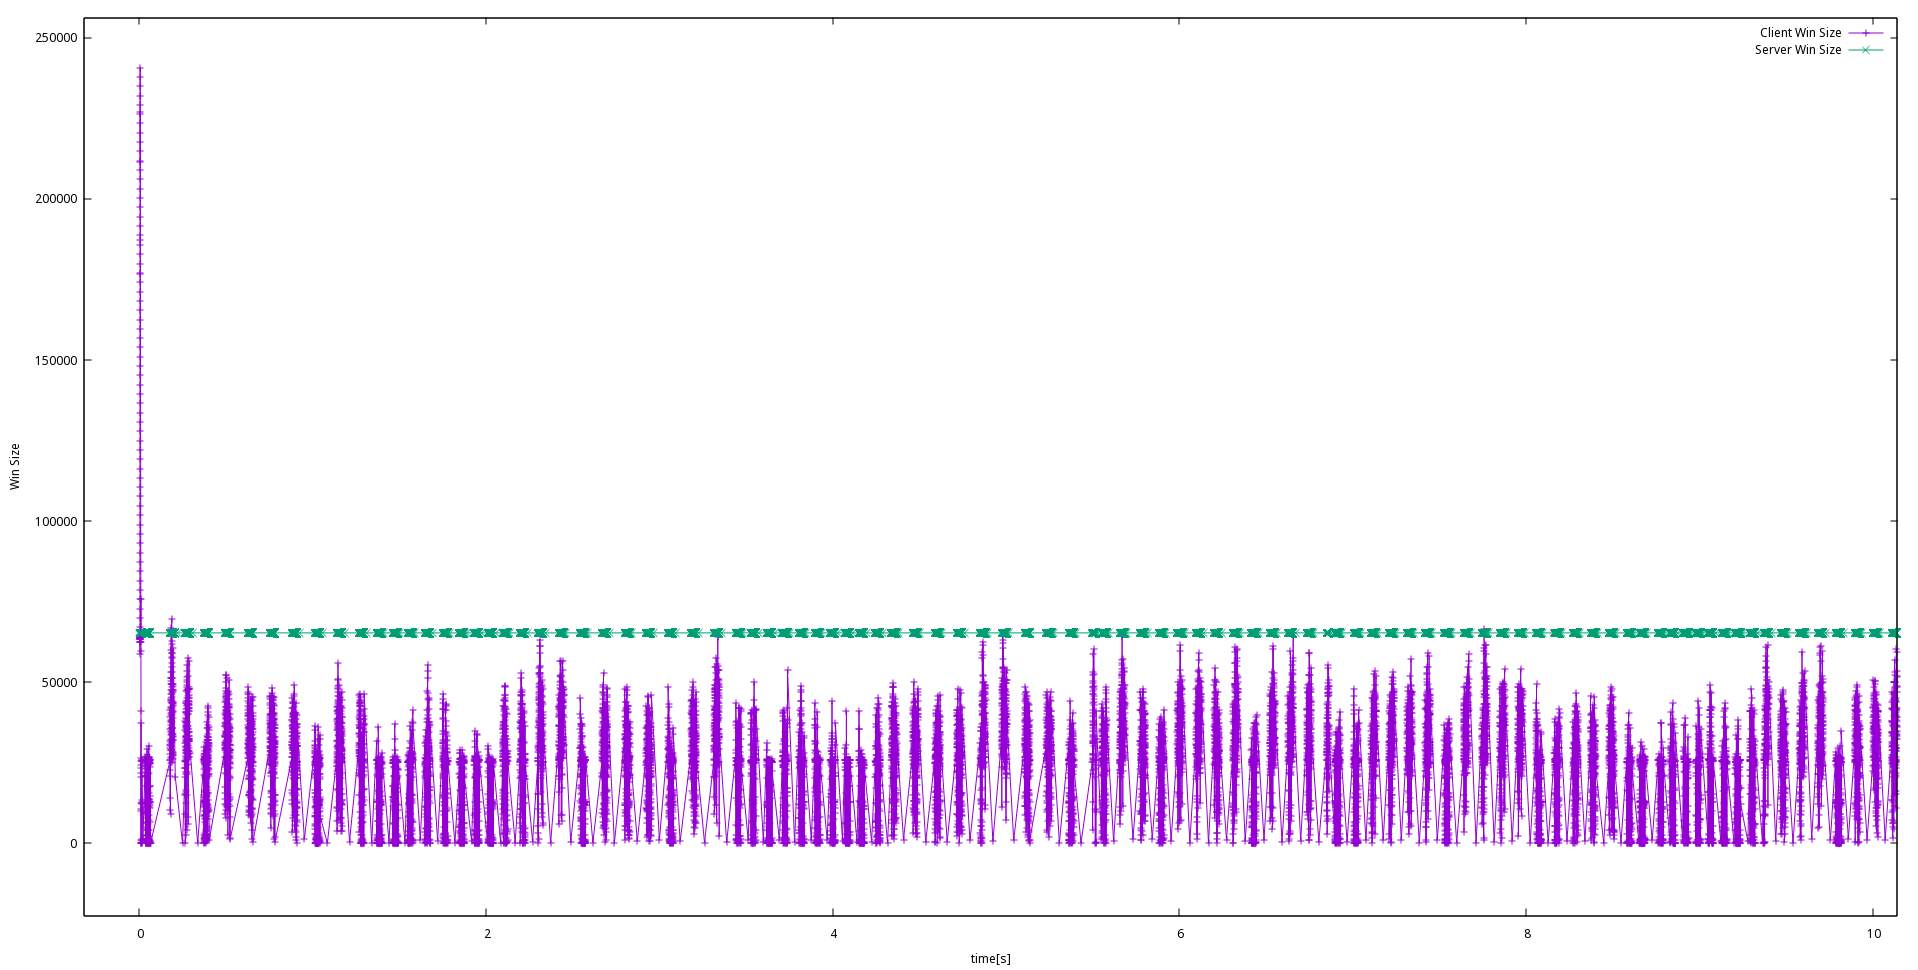
\includegraphics[width=0.50\textwidth]{rwnd_1-2.png}
    \caption{Client and Server RWND during phase 1-2}
    \label{fig:rwnd_1-2}
\end{figure}
\begin{figure}[H]
    \centering
    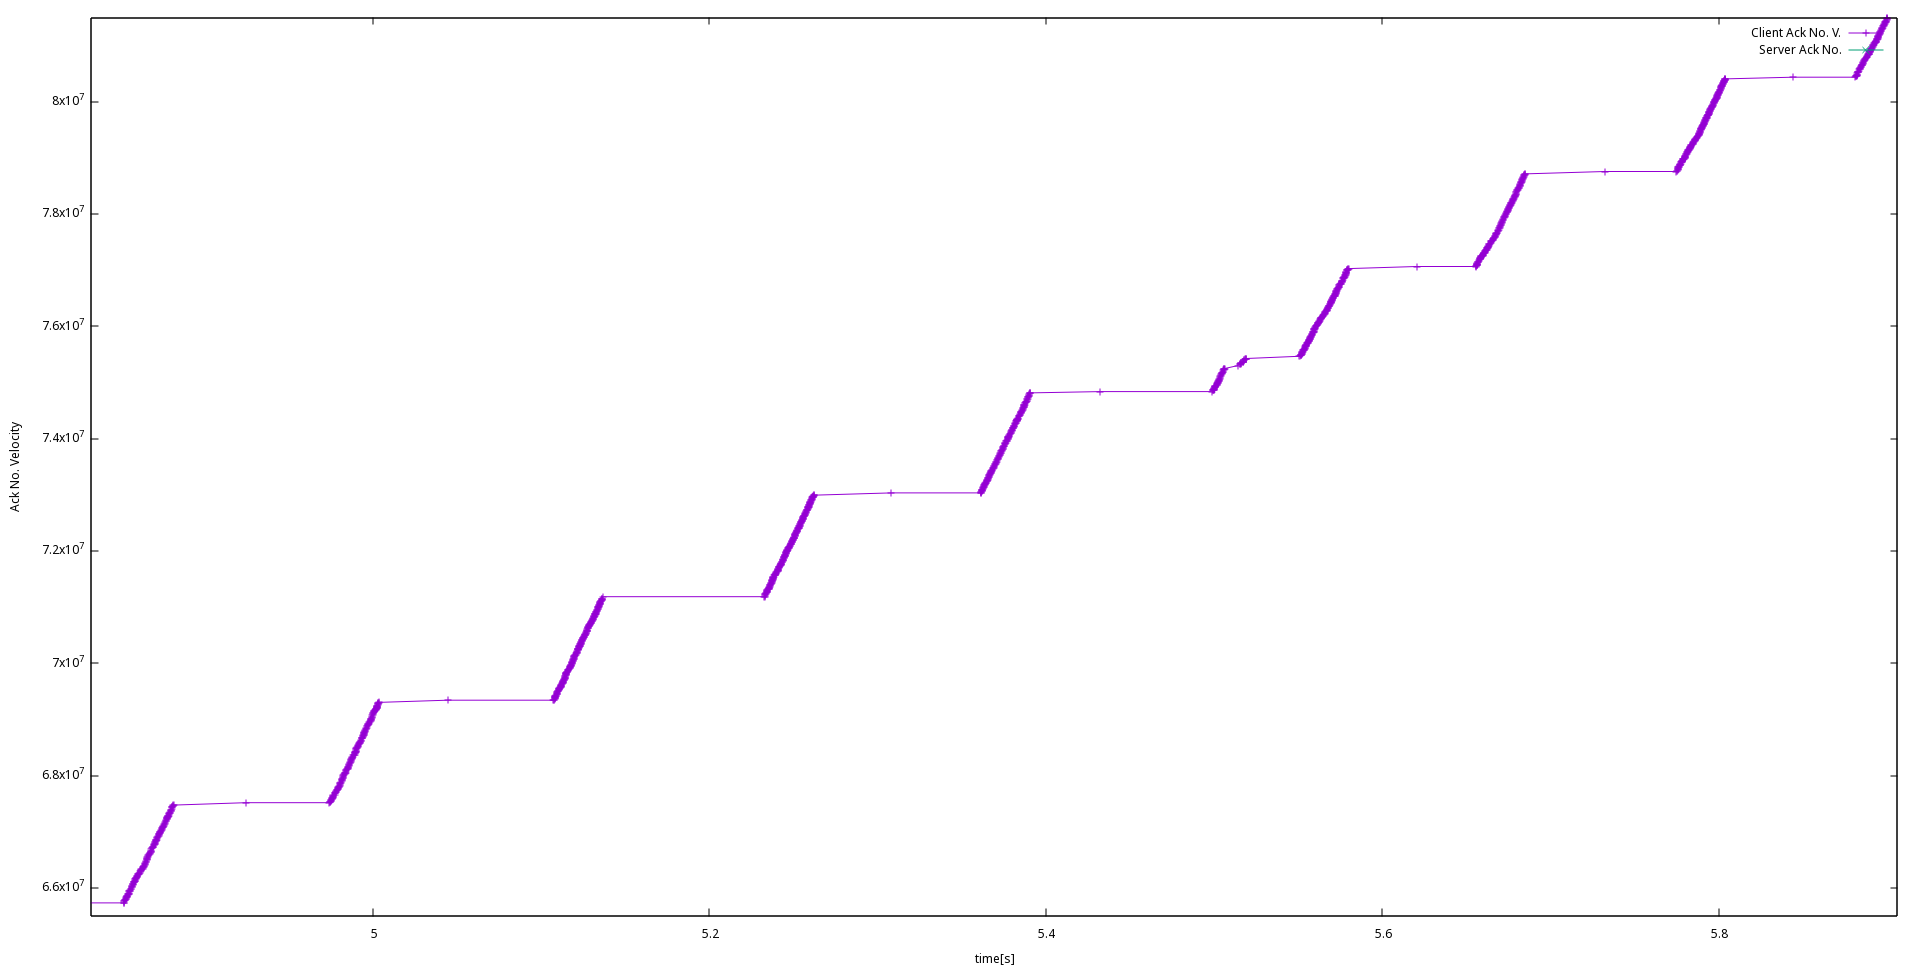
\includegraphics[width=0.50\linewidth]{step_1-2.png}
    \caption{A microscopic view of the first two phases}
    \label{fig:step_1-2}
\end{figure}

A last scenario can be observed by zooming a lot on our server seq number graph as shown in graph \ref{fig:step_1-2}, periodically the server after sending a variable quantity of data based on implementation parameters and current connection status interrupts is communication before saturating the last advertised \verb|RWND|. If the corresponding \verb|ACK| from the client doesn't arrive in the next 10-15ms the server re-transmits the last packet (marked as \textbf{TCP Retransmission} by Wireshark and highlighted as the isolated segment in nearly each plateau of the graph \ref{fig:step_1-2}) in order to force the client to answer , something similar to what we'll see in the Keep-Alive section: by observing the \verb|ctrl+c| phase of the experiment we can assume that the re-transmission timer is parameterized also around the \verb|RWND| of the other host because in that experience, in which the client receiving window is a lot bigger, we don't have retransmission even if we have waiting time before some \verb|ACK| longer than 30ms and that's the probable reason because some plateau has no TCP retransmission.

\subsection{System Overloading}
This experiment aims to provide evidence of a \textbf{decreased throughput} when the system is begin overloaded.

In order to do this we opened two terminals, in one of them a openssl benchmark was run, while on the other a telnet session was opened with the Chargen server. The reason why we used openssl is because by launching the benchmark mode, openssl starts performing as many cryptographic operations as possible, because they are very demanding in terms of CPU power required, the whole system is affected by this operations. At the 15th second we stopped the openssl program, the Figure~\ref{fig:sys-overloading} shows the pace of the graph, shortly after we see an increase in the slope of the Client Ack No., and further supported by the time derivative of the Ack, which shows greater peaks after the 15 seconds threshold.

We can clearly state after this experiment the fact that we did not see any noticeable change in the original experiment while performing a terminal window resizing in Subsection~\ref{ssec:resizing-the-terminal-window}, is totally justified by the fact that the PC we test were able to handle a simple window resizing.


 
\subsection{Opening the Telnet terminal}
\begin{figure}[H]
    \centering
    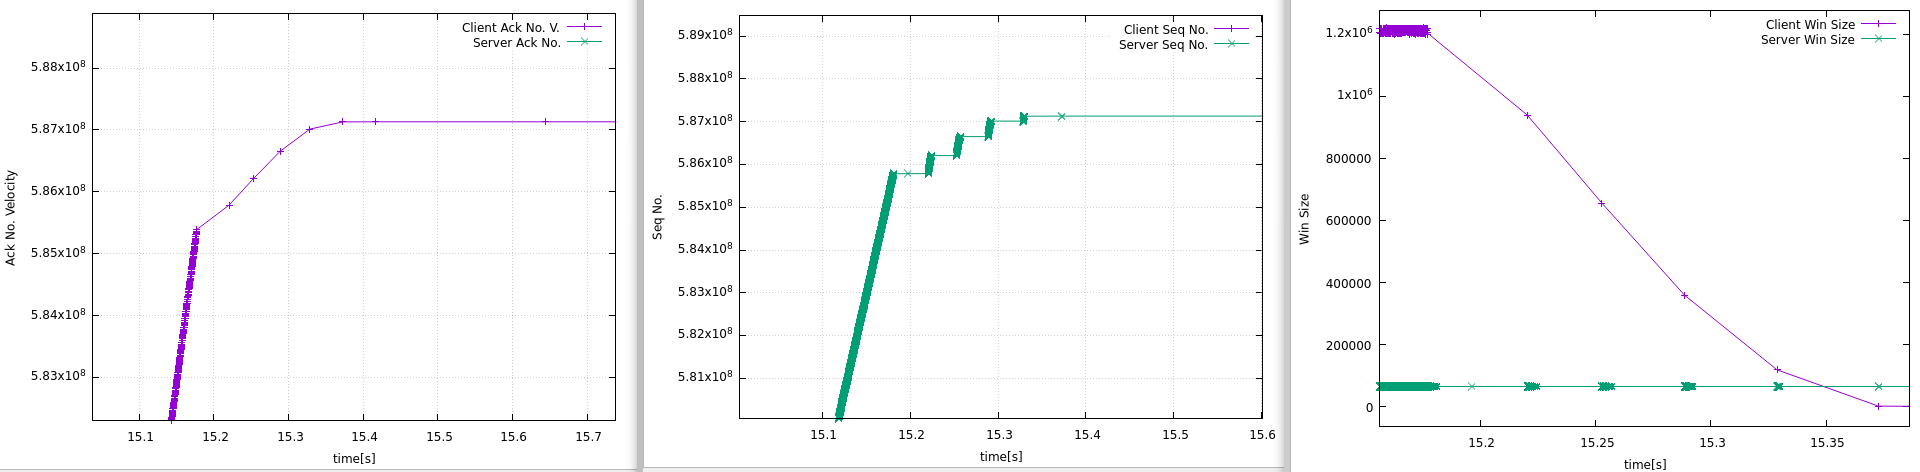
\includegraphics[width=1\textwidth]{telnet-term-opening-closeup.png}
    \caption{Closeup during the terminal opening}
    \label{fig:telnet-term-opening-closeup}
\end{figure}
When the key combination \verb|^]| gets pressed, the client enters into the \verb|command mode| of Telnet; at this point, the client starts sending the server \texttt{ACK} segments with always decreasing window size, clearly illustrated in the third graph, in the end the client sends an \texttt{ACK} with \texttt{win=0}, which means that the client has put the connection on hold and doesn't want to receive any more data from the server. This could be due to the fact that when the telnet terminal is opened all the data to the client cannot be displayed to the screen so TCP is not able to pass this information from its cache to the telnet application and the window slowly fills up, up to the point where it is completely full. Only when the client will press Enter from the telnet terminal, the application will start printing again character on the screen thus start consuming the TCP buffer, and again increase its window size. Now the problem is: \textit{What happens in the time interval between when the telnet terminal is opened and it gets closed?}

\subsection{The Keep-Alive phase}\label{ssec:the-keep-alive-problem}
\begin{figure}[H]
    \centering
    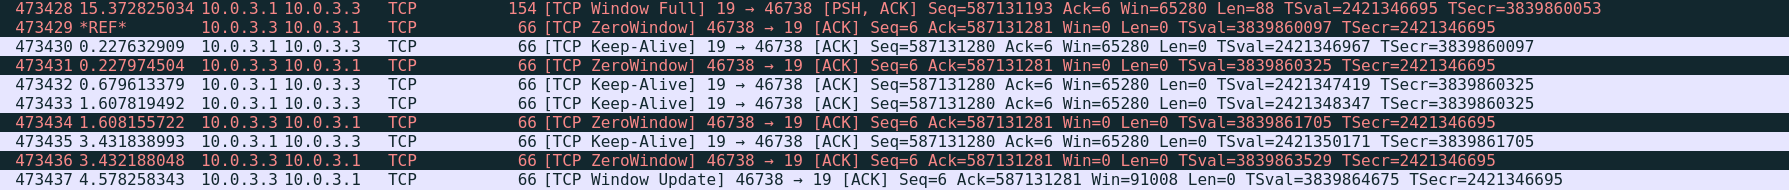
\includegraphics[width=1\textwidth]{keep-alive.png}
    \caption{Server tries to keep alive the connection}
    \label{fig:keep-alive}
\end{figure}
This figure has the time of the segments referencing the \texttt{TCP ZeroWindow} segment. By doing that it is possible to see how the server is able to keep alive the connection.

As we can see from the Figure~\ref{fig:keep-alive} when the client send the \texttt{ZeroWindow} segment the server goes into \textbf{keep-alive mode}, this is done by sending a special kind of segments, that are able to force an answer from the client without sending any new data, that are called \textbf{TCP Keep-Alive} by Wireshark. This segments don't carry any data but their sequence number is peculiar, it corresponds to the next Sequence Number minus 1 (e.g. in this case, after the first \verb|ZeroWindow|, the next sequence no. would be the sequence number of the last segment plus its length: $587131193 + 88 = 587131281$). This is able to force an answer from the client which will acknowledge the fact that the server already sent this bytes along its Window size which may be updated or not.

This probe segments are not sent with the same time interval, but it \textbf{increases} over time, from the trace is not very clear what is the multiplying factor, it start at around 3x and it does look approaching 2x.  

Reading the TCP man pages it is clear also the keep-alive mode has a timeout which by default is 7200 seconds (2 hours), and all the TCP parameters can be located at \verb|/proc/sys/net/|. The file which gives out the keep-alive timeout is \verb|tcp_keepalive_time|.

\section{Cable-Cut}
\begin{figure}[H]
    \centering
    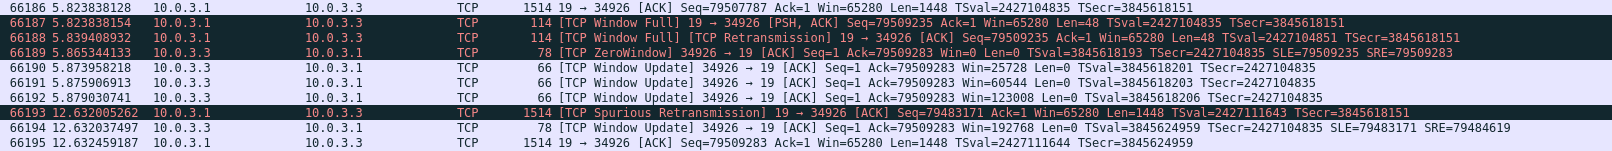
\includegraphics[width=0.9\textwidth]{cable-client.png}
    \caption{Interface of the client during cable cut}
    \label{fig:cable-client}
\end{figure}
\begin{figure}[H]
    \centering
    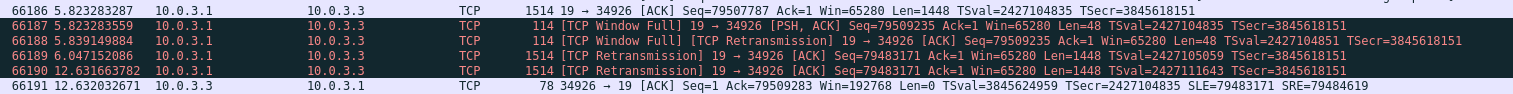
\includegraphics[width=0.9\textwidth]{cable-server.png}
    \caption{Interface of the server during cable cut}
    \label{fig:cable-server}
\end{figure}
Another experiment we performed was to try and cut the cable while the connection between the client and the server was already opened.

What happened was that unlike the Subsection~\ref{ssec:the-keep-alive-problem}, where the server tried to keep-alive the connection by sending the client special segments, the server only tried to to do one retransmission after the cable was cut, because the first retransmission was received by the client, also the client tried to send three Ack, but none of them reached the server, during this period neither the server nor the client sent any other segments. Only after the cable was put in place the server sent another retransmission to the client and the connection continued just as normal as before.



\pagebreak
\section{Appendix}
\subsection{Chargen captures}
\begin{figure}[H]
    \centering
    \begin{subfigure}[b]{0.4\textwidth}
        \centering
        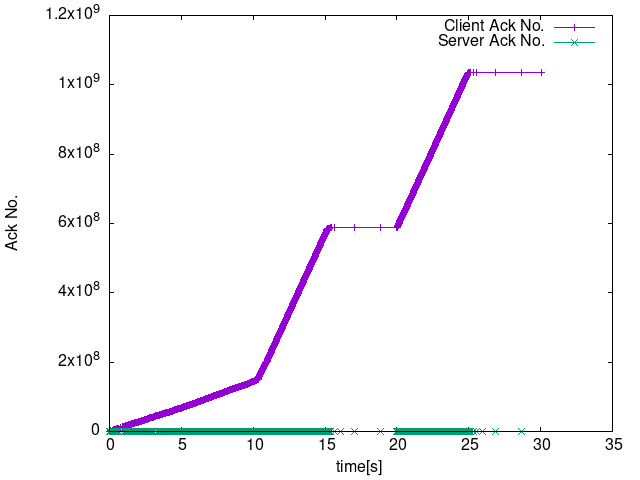
\includegraphics[width=\textwidth]{base_test/ack.png}
        \caption{Client/Server Ack No.}
        \label{fig:ack}
    \end{subfigure}
    \hfill
    \begin{subfigure}[b]{0.4\textwidth}
        \centering
        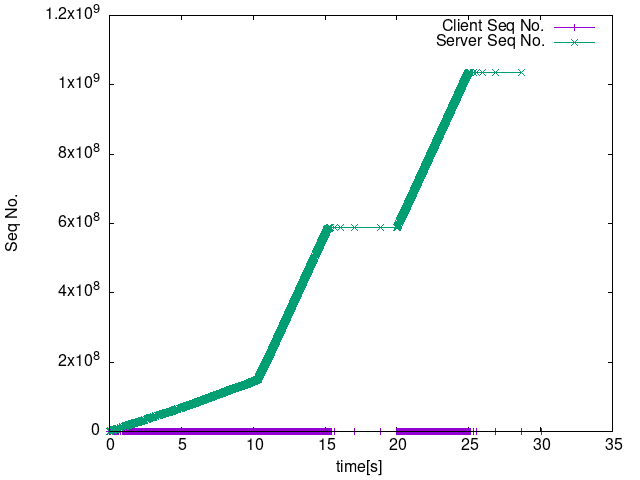
\includegraphics[width=\textwidth]{base_test/seq.png}
        \caption{Client/Server Seq No.}
        \label{fig:seq}
    \end{subfigure}
    \hfill
        \begin{subfigure}[b]{0.4\textwidth}
        \centering
        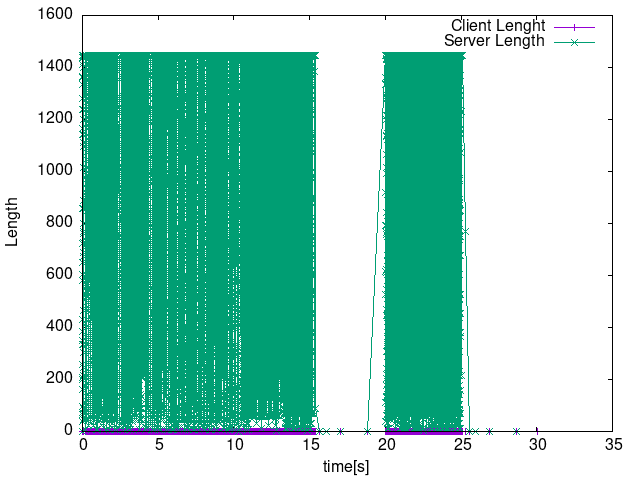
\includegraphics[width=\textwidth]{base_test/len.png}
        \caption{Client/Server Len}
        \label{fig:len}
    \end{subfigure}
    \hfill
    \begin{subfigure}[b]{0.4\textwidth}
        \centering
        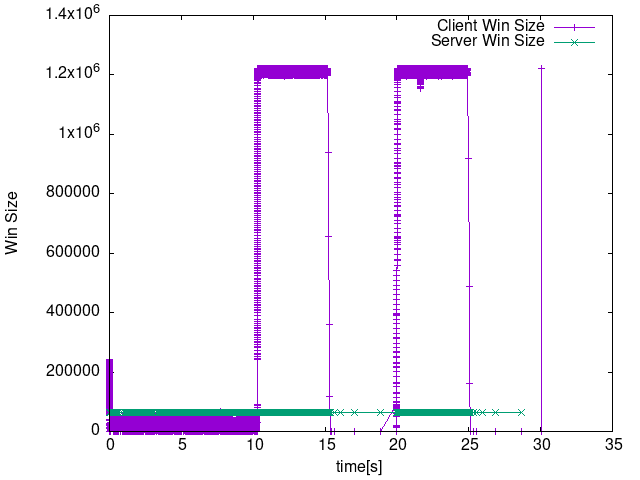
\includegraphics[width=\textwidth]{base_test/win.png}
        \caption{Client/Server Win}
        \label{fig:win}
    \end{subfigure}
    \hfill
    \begin{subfigure}[b]{0.4\textwidth}
        \centering
        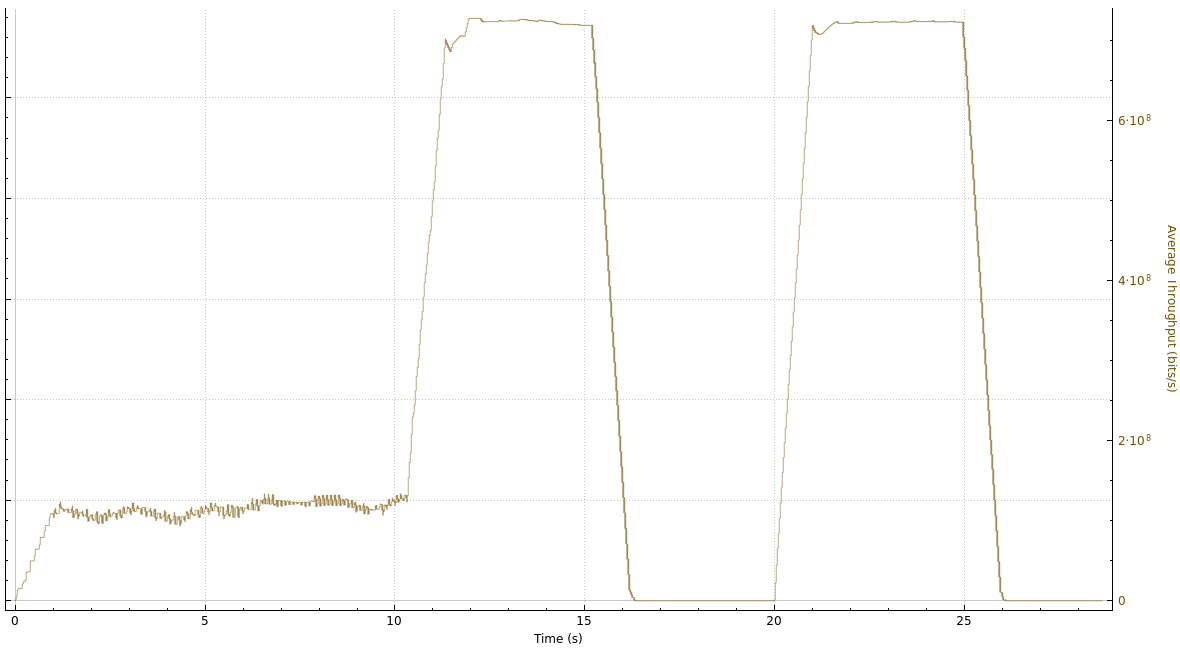
\includegraphics[width=\textwidth]{base_test/throughput.png}
        \caption{Server Throughput}
        \label{fig:throughput}
    \end{subfigure} 
    \caption{Chargen Capture}
\end{figure}

\subsection{Handshake Segments}
\begin{figure}[H]
    \centering
    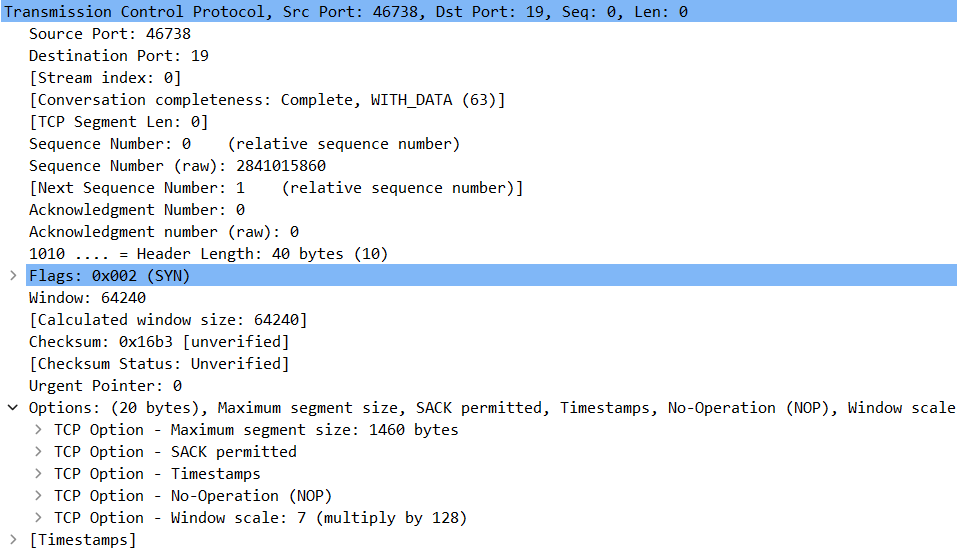
\includegraphics[width=0.50\textwidth]{TWH_Syn.png}
    \caption{SYN fragment}
    \label{fig:syn_fragment}
\end{figure}

\begin{figure}[H]
    \centering
    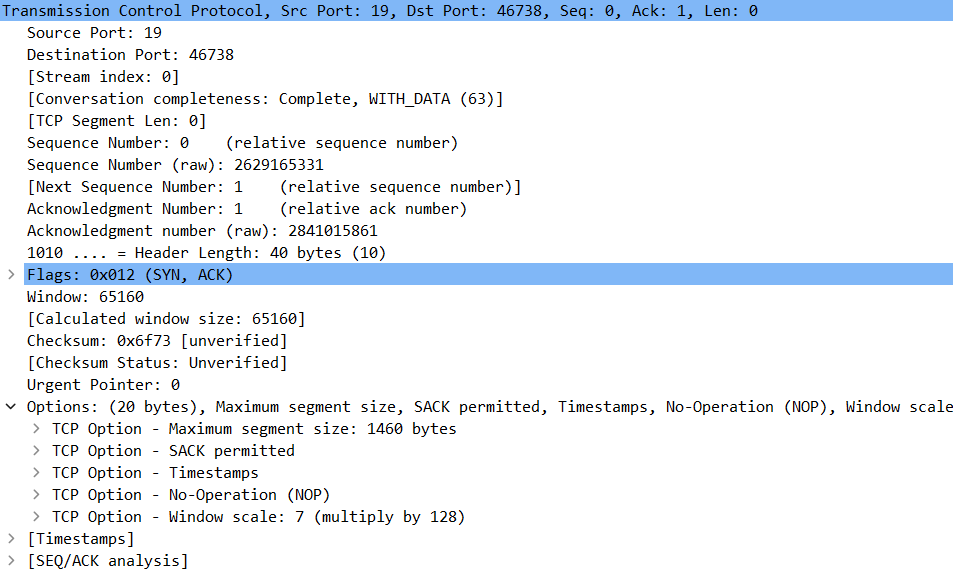
\includegraphics[width=0.50\textwidth]{TWH_SynAck.png}
    \caption{SYN/ACK fragment}
    \label{fig:synack_fragment}
\end{figure}

\begin{figure}[H]
    \centering
    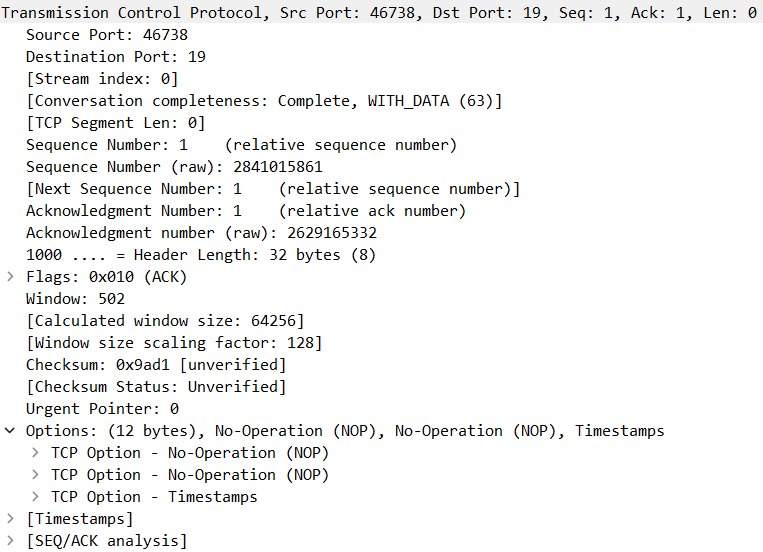
\includegraphics[width=0.50\textwidth]{TWH_Ack.png}
    \caption{ACK fragment}
    \label{fig:ack_fragment}
\end{figure}

\subsection{Throughput}
\begin{figure}[H]
    \centering
    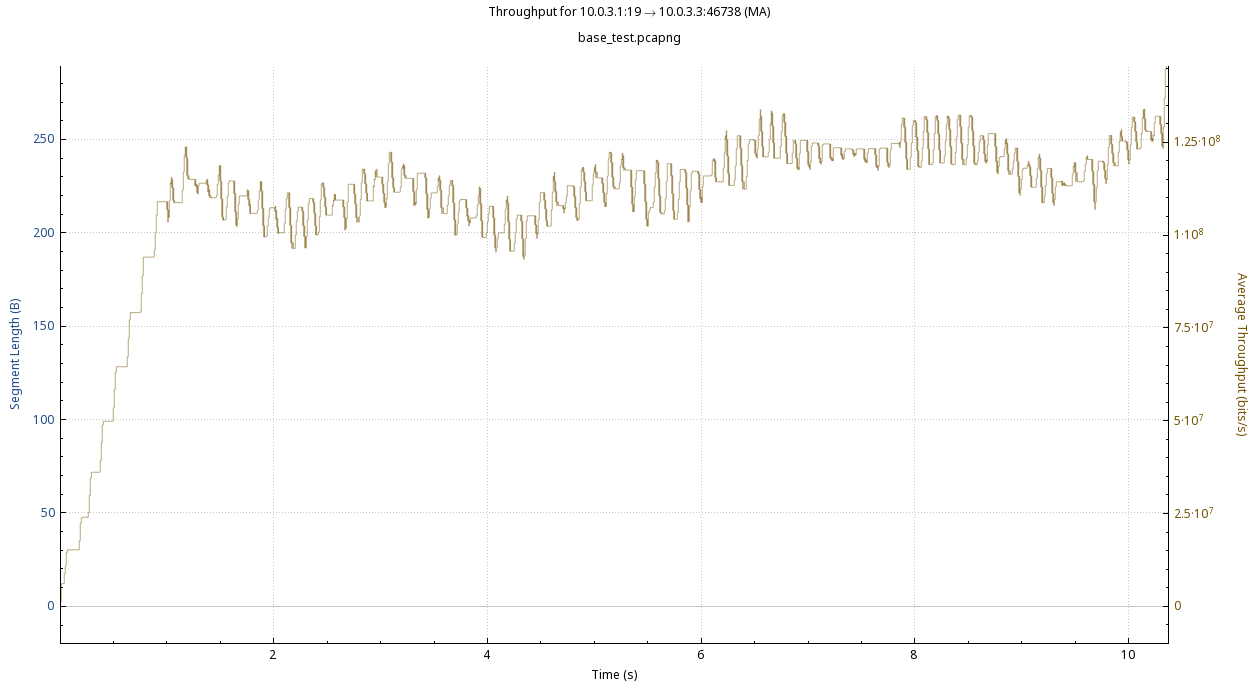
\includegraphics[width=0.50\textwidth]{throughput_phase1-2.png}
    \caption{Throughput during phase 1-2}
    \label{fig:throughput_1-2}
\end{figure}

\subsection{System Overloading}
\begin{figure}[H]
    \centering
    \begin{subfigure}[b]{0.4\textwidth}
        \centering
        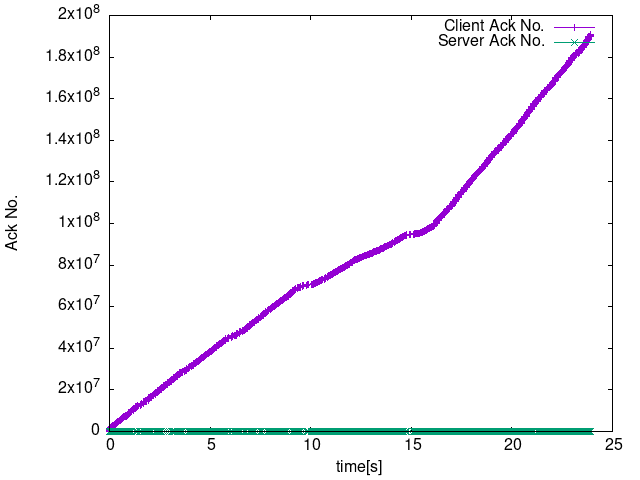
\includegraphics[width=\textwidth]{overload-ack.png}
        \caption{Client Acknowledge}
    \end{subfigure}
    \hfill
    \begin{subfigure}[b]{0.4\textwidth}
        \centering
        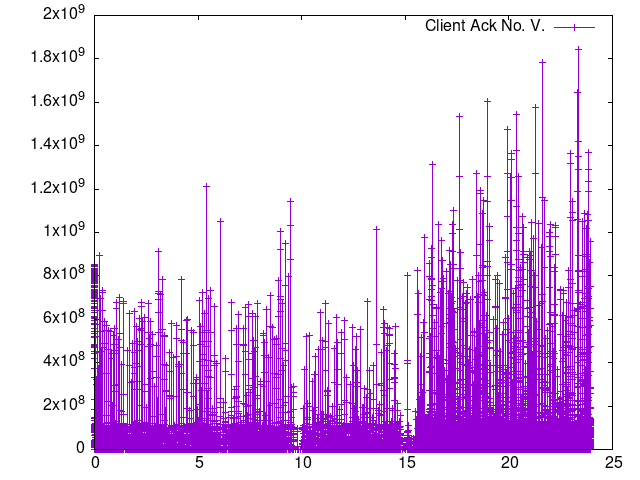
\includegraphics[width=\textwidth]{overload-ack-vel.png}
        \caption{Client Acknowledge Velocity}
    \end{subfigure}
    \caption{System overloading client ACK graphs}
    \label{fig:sys-overloading}
\end{figure}

\subsection{Script for image generation}
\begin{lstlisting}[language=bash]
#!/bin/sh

for arg in $@; do
	case $arg in
		-d|--dynamic)
			DYNAMIC=1
			shift
			;;
		-*|--*)
			echo "Invalid option!"
			exit 1
			;;
		*)
			;;
	esac
done

if [ ! -f $1 ] || [ -z $1 ]; then
	echo "$0: Wrong params!"
	exit 1
fi

echo "generating client values..."
# Generate client time and values, remove first ACK packet
tail -n +3 $1 | grep -P "> *19" | tr -s "\"" "," | tr "," " " | tr -s " " | cut -d " " -f 3 > client_time.txt
tail -n +3 $1 | grep -P "> *19" | tr -s "\"" "," | tr "," " " | tr -s " " | grep -oP "(?<=Ack=)([^ ]*)" > client_ack.txt
tail -n +3 $1 | grep -P "> *19" | tr -s "\"" "," | tr "," " " | tr -s " " | grep -oP "(?<=Seq=)([^ ]*)" > client_seq.txt
tail -n +3 $1 | grep -P "> *19" | tr -s "\"" "," | tr "," " " | tr -s " " | grep -oP "(?<=Len=)([^ ]*)" > client_len.txt
tail -n +3 $1 | grep -P "> *19" | tr -s "\"" "," | tr "," " " | tr -s " " | grep -oP "(?<=Win=)([^ ]*)" > client_win.txt

paste client_time.txt client_ack.txt > client_ta.txt
paste client_time.txt client_seq.txt > client_ts.txt
paste client_time.txt client_win.txt > client_tw.txt
paste client_time.txt client_len.txt > client_tl.txt

echo "generating server values..."
# Generate server time and values
tail -n +2 $1 | grep -P "19 *>" | tr -s "\"" "," | tr "," " " | tr -s " " | cut -d " " -f 3 > server_time.txt
tail -n +2 $1 | grep -P "19 *>" | tr -s "\"" "," | tr "," " " | tr -s " " | grep -oP "(?<=Ack=)([^ ]*)" > server_ack.txt
tail -n +2 $1 | grep -P "19 *>" | tr -s "\"" "," | tr "," " " | tr -s " " | grep -oP "(?<=Seq=)([^ ]*)" > server_seq.txt
tail -n +2 $1 | grep -P "19 *>" | tr -s "\"" "," | tr "," " " | tr -s " " | grep -oP "(?<=Len=)([^ ]*)" > server_len.txt
tail -n +2 $1 | grep -P "19 *>" | tr -s "\"" "," | tr "," " " | tr -s " " | grep -oP "(?<=Win=)([^ ]*)" > server_win.txt

paste server_time.txt server_ack.txt > server_ta.txt
paste server_time.txt server_seq.txt > server_ts.txt
paste server_time.txt server_win.txt > server_tw.txt
paste server_time.txt server_len.txt > server_tl.txt

echo "plotting..."

if [ $DYNAMIC ]; then
	echo "Ack..."
	gnuplot <<EOF &
set xlabel "time[s]"
set ylabel "Ack No. Velocity"
plot "client_ta.txt" using 1:2 title "Client Ack No." with linespoint, "server_ta.txt" using 1:2 title "Server Ack No." with linespoint
pause 9999
EOF

	echo "Ack Velocity..."
	gnuplot <<EOF &
set xlabel "time[s]"
set ylabel "Ack No."
dx(x) = (x0=x1, x1=column(x), (x0 + x1) / 2.)
dy(y) = (y0=y1, y1=column(y), (y1 - y0)/(x1 - x0))
plot x1=y1=NaN "client_ta.txt" using (dx(1)):(dy(2))  title "Client Ack No. V." with linespoint
pause 9999
EOF

	echo "Seq..."
	gnuplot <<EOF &
set xlabel "time[s]"
set ylabel "Seq No."
plot "client_ts.txt" using 1:2 title "Client Seq No." with linespoint, "server_ts.txt" using 1:2 title "Server Seq No." with linespoint
pause 9999
EOF

	echo "Win..."
	gnuplot <<EOF &
set xlabel "time[s]"
set ylabel "Win Size"
plot "client_tw.txt" using 1:2 title "Client Win Size" with linespoint, "server_tw.txt" using 1:2 title "Server Win Size" with linespoint
pause 9999
EOF

	echo "Len..."
	gnuplot <<EOF &
set xlabel "time[s]"
set ylabel "Length"
plot "client_tl.txt" using 1:2 title "Client Length" with linespoint, "server_tl.txt" using 1:2 title "Server Length" with linespoint
pause 9999
EOF

else
	echo "Ack..."
	gnuplot -persist <<EOF
set term png
set output "ack.png"
set xlabel "time[s]"
set ylabel "Ack No."
plot "client_ta.txt" using 1:2 title "Client Ack No." with linespoint, "server_ta.txt" using 1:2 title "Server Ack No." with linespoint
EOF

	echo "Ack Velocity..."
	gnuplot -persist <<EOF
set term png
set output "ack-vel.png"
dx(x) = (x0=x1, x1=column(x), (x0 + x1) / 2.)
dy(y) = (y0=y1, y1=column(y), (y1 - y0)/(x1 - x0))
plot x1=y1=NaN "client_ta.txt" using (dx(1)):(dy(2))  title "Client Ack No. V." with linespoint
EOF

	echo "Seq..."
	gnuplot -persist <<EOF
set term png
set output "seq.png"
set xlabel "time[s]"
set ylabel "Seq No."
plot "client_ts.txt" using 1:2 title "Client Seq No." with linespoint, "server_ts.txt" using 1:2 title "Server Seq No." with linespoint
EOF

	echo "Win..."
	gnuplot -persist <<EOF
set term png
set output "win.png"
set xlabel "time[s]"
set ylabel "Win Size"
plot "client_tw.txt" using 1:2 title "Client Win Size" with linespoint, "server_tw.txt" using 1:2 title "Server Win Size" with linespoint
EOF

	echo "Len..."
	gnuplot -persist <<EOF
set term png
set output "len.png"
set xlabel "time[s]"
set ylabel "Length"
plot "client_tl.txt" using 1:2 title "Client Lenght" with linespoint, "server_tl.txt" using 1:2 title "Server Length" with linespoint
EOF
fi

echo "Finished"
\end{lstlisting}

\end{document}